\chapter{Introduction}\label{ch:introduction}
Google Cloud Platform, Amazon Web Service and Microsoft Azure provide a service to users with computer programs that
are too large, difficult or time consuming to be run on standard computer. User can request a fixed amount of resources
to run the program, e.g. cpu cores, RAM, hard drive space, bandwidth, etc. However,
this can create bottlenecks on certain resources due to large numbers of resource requests preventing other jobs from
running. This problem is particularly relevant in edge cloud computing as servers
are small thus making the demand on resources much greater. This project considers the case where the user states
the total resource requirements for the program instead of the standard procedure that user request a fixed
amount of resources. This allows the cloud provider the ability to balance resource demand as it has
complete knowledge of all user's requirements and can flexibly change the amount of resources allocated to each
task. This can prevent bottlenecks through proper balances of resources allowing more tasks to run simultaneously
and can also lower the price due to there being a lower overall demand on resources.

Recently, cloud computing~\citep{cloud_cite} has become a popular solution for remotely running data-intensive applications.
But for some problem domains, it is not possible to use large cloud providers, for example running highly delay-sensitive
tasks or where connectivity to the cloud is intermittent. Mobile edge computing~\citep{mobile_edge_survey} has emerged as a
complementary paradigm to allow for small data-centers, close to users, to execute tasks. These data centers are known
as edge clouds.

Disaster response, smart cities and Internet-of-things (IoT) are popular technologies that utilise mobile edge
computing due to the use of ability to process small programs locally with low latency. For smart cities, this
allows for the possibly of smart intersections with the use of road-side sensors or smart traffic lights based
on cameras to minimise the waiting times~\citep{smart_cities_traffic_lights}. Or for the police to analysis
CCTV footage to spot suspicious behaviour or to track people between cameras~\citep{Sreenu2019}. In the case
of disaster response, maps can be produced using autonomous vehicles sensors to be used in the search for potential
victims and support responders~\citep{smart_disaster_management}.

To compute these task, several types of resources are required included communication bandwidth, computational power
and data storage resources~\citep{vaji_infocom}. Tasks will have a deadline such that the program must be completed
before this point and a private value. This value is depend on the program itself and its value to the owner, .e.g analysis air pollution is
less important than preventing traffic jams at rush hour or tracking a criminal on the run. This project is interested
in allocated task to servers to maximise the social welfare (sum of all allocated task values) over time. But due to users being
self-interested, they may behave strategically~\citep{Bi2019} or prefer to not reveal their value publicity~\citep{Pai2013}.

The shortcoming of existing work for resource allocation in edge cloud computing \citep{vaji_infocom, Bi2019}
has the assumption that tasks have fixed resource requirements. However, flexibility is possible in practise
with how resources are allocaed to each task. For example, the allocated bandwidth for loading the program is
proportional to the time taken to load the program. This is true of also the computational requirements and
for sending results back to the user. This project investigates flexible allocation of resource and pricing
mechanisms when task arrive over time and have private values.

\chapter{Related Works}\label{ch:related-works}
Due to the novel approach for resource allocation in cloud computing, there is few papers that allow for flexible
resource allocation. However there is a considerable amount of research in the area of resource allocation and
pricing in cloud computing, some of which use auction mechanisms to deal with competition~\cite{KUMAR2017234,Zhang2017,Du2019,Bi2019}.
In Section~\ref{sec:related-work-cloud-computing} considers the previously related work for flexible resource
allocation in cloud computing and Section~\ref{sec:related-work-reinforcement-learning} consider recent
work in the field of reinforcement learning.

\section{Related work in Cloud computing}\label{sec:related-work-cloud-computing}
A majority of the approaches for pricing and resource allocation in cloud computing require users to request a
fixed amount of certain resource with the cloud provider having no control over the resources only the servers that the
task was allocated to~\citep{KUMAR2017234,Zhang2017,Du2019,Bi2019}. The flexible approach that this project
assumed has only been considered in~\cite{FlexibleResourceAllocation} that allows the server to distribute its resources
more efficiently based on each task's requirements. The primary difference between this project and that paper is that this
project considers the addition of time allowing for resource speed to change over time and that there are task stages.

Previous work by \cite{FlexibleResourceAllocation} considers three solutions to a single-shot problem case,
a greedy algorithm to quickly approximate a solution to maximise the social welfare and two auction mechanisms as server
are normally paid for usage of their resources. The greedy algorithm is a polynomial time algorithm that will find solution
within $\frac{1}{n}$ of the optimal social welfare.
This is done through the use of modular heuristics for ordering the task by density then for each task, select a server
based on available resource on each servers then to allocate resources that minimises a resource heuristics.
Using certain heuristics, the greedy algorithm achieves at least 90\% of the optimal solution and 20\% more than optimal
solution for fixed resource equivalent problems. A new distributed iterative auction was developed that use a reverse vcg
principle to calculate a task price that meant that a task didnt need to reveal its private value also that the
auction could be run in a decentralised way. This means that the auction is budget balanced however it is not
economically efficient or incentive compatible. The third algorithm is an implementation of a single parameter
auctions~\citep{nisan2007algorithmic_critical_value} using the greedy algorithm to find the critical value of a task.
Using this mechanism with a monotonic value density heuristic means that the auction is incentive compatible.

Other closely related work on resource allocation in edge clouds~\cite{vaji_infocom} considers both the placement of
code/data needed to run a specific task, as well as the scheduling of tasks to different edge clouds. The goal there
is to maximize the expected rate of successfully accomplished tasks over time. Our work is different both in the setup
and the objective function. Our objective is to maximize the value over all tasks. In terms of the setup, they assume
that data/code can be shared and they do not consider the elasticity of resources.

\section{Related work in Reinforcement learning}\label{sec:related-work-reinforcement-learning}
Supervised learning allows for the training of agents to converge towards a truth value while unsupervised learning
allows for the training of agents find pattern for data where no-truth value exist. Reinforcement learning works in the
middle ground where truth value exist but are unknown so agent will interact with an environment that depending on certain
actions will result in being rewarded. Using this resulted in the first successful "machine-learning" agent in 1959 with
TD-Checking~\citep{samuel1988some} where the truth value was the difference in two "neighbouring" checkers boards. Temporal difference,
Q-learning, SARSA and other were early training methods for agents using reinforcement learning.

The work of \cite{atari} developed the usage of these methods much further by coupling them with deep neural network
allowing an agent to be trained using the same algorithm to achieve state-of-the-art in 6 of 7 games tried and superhuman scores in
3. This recent work has reinvigorated to the area primarily due to the availability of data to be used and the computational power
available. This has allowed \cite{silver2017mastering} to achieve mastery of the game of Go learning from no human expert
to beat the world champion 4 games to 1. With following work expanding to other games like DOTA 2~\citep{OpenAI_dota} beating the
world champions and Starcraft 2~\citep{starcraft2} becoming in the top 2\% world wide.

\chapter{Proposed solution}\label{ch:proposed_solution}
The problem case presented in Chapter~\ref{ch:introduction} has two stages: auction and resource allocation.
These stages are discussed in sections~\ref{sec:auction_solution} and~\ref{sec:resource_allocation}
respectively.

\section{Optimisation problem}
A sketch of the system is shown in Fig.~\ref{fig:system_model}.
We assume that in the system there is a set of $I = \{1,2,\ldots,\left|I\right|\}$ servers are heterogeneous in all
characters. Each server has a fixed availability of resources: storage for the code/data needed to run a task
(e.g., measured in GB), computation capacity in terms of CPU cycles per time interval (e.g., measured in FLOP/s),
and communication bandwidth to receive the data and to send back the results of the task after execution (e.g., measured in Mbit/s).
We denote these resources for server $i$: the storage capacity as $S_i$, computation capacity as $W_i$, and the communication capacity as $R_i$.

\begin{figure}
    \centering
    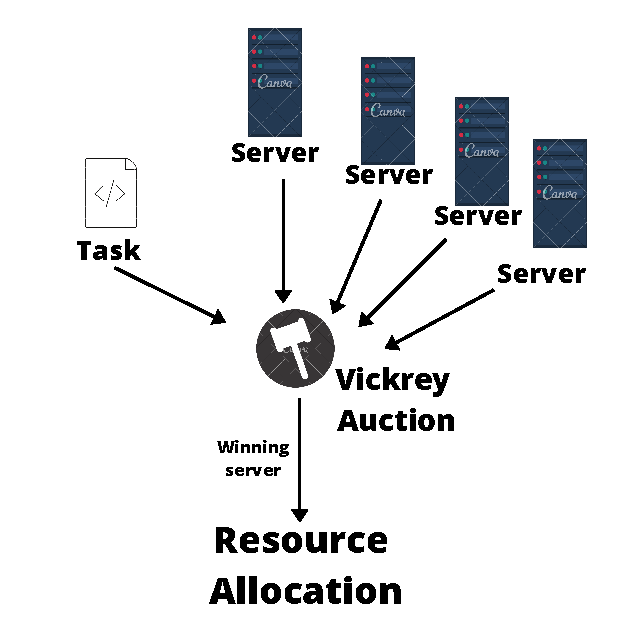
\includegraphics{extra/system_model.pdf}
    \caption{System model}
    \label{fig:system_model}
\end{figure}

There is a set $J = \{1,2,\ldots,\left| J \right|\}$ of  different tasks that require service from one of the servers
in set $I = \{1,2,\ldots, \left| I \right|\}$. To run any of these tasks on a server requires storing the appropriate
code/data on the same server. These could be, for example, a set of images, videos or CNN layers in identification
tasks. The storage size of task $j$ is denoted as $s_j$ with the rate at which the program is transferred to the server
$i$ at time $t$ being $s^{'}_{i,j,t}$. For a task to be computed successfully, it must fetch and execute instructions
on a CPU. We consider the total number of CPU cycles required for the program to be $w_j$, where the rate at which the
CPU cycles are assigned to the task on server $i$ at time $t$ is $w^{'}_{i,j,t}$. Finally, after the task is run and
the results obtained, the latter need to be sent back to the user. The size of the results for task $j$ is denoted with
$r_j$, and the rate at which they are sent back to the user is $r^{'}_{i,j,t}$ on server $i$ at time $t$. Every task
has a beginning time, denoted by $b_j$ and a deadline, denoted by $d_j$. This is the maximum time for the task to be
completed in order for the user to derive its value. This time includes: the time required to send the data/code to the
server, run it on the server, and get back the results. Therefore for the task to be successfully completed, it must
completed fulfill the constraint in equation~\eqref{eq:deadline}. These operations must occur in order (loading,
computing then sending of results) as a server couldn't compute a task that was not fully loaded on the machine.

\begin{align}
    \frac{s_j}{\sum^{d_j}_{t=b_j} s^{'}_{i,j,t}} + \frac{w_j}{\sum^{d_j}_{t=b_j} w^{'}_{i,j,t}}  +
    \frac{r_j}{\sum^{d_j}_{t=b_j} r^{'}_{i,j,t}} \leq d_j && \forall{j \in J}  \label{eq:deadline}
\end{align}

As server have limited capacity, the total resource usages for all tasks running on a server must be capped.
The storage constraint (equation~\eqref{eq:server_storage_capacity}) is unique as the previous amount
loaded in kept till the end of a program on server. While the computation capacity
(equation~\eqref{eq:server_computation_capacity} is the sum of compute used by all of the tasks on a server $i$ at time $t$ and the
bandwidth capacity (equation~\eqref{eq:server_bandwidth_capacity}) is the sum of loading and sending usages by tasks.
\begin{align}
    \sum_{j \in J} \left(\sum^{d_j}_{t=b_j} s^{'}_{i,j,t} \right) \leq S_i, && \forall{i \in I} \label{eq:server_storage_capacity} \\
    \sum_{j \in J} w^{'}_{i,j,t} \leq W_i, && \forall{i \in I, t \in T} \label{eq:server_computation_capacity} \\
    \sum_{j \in J} s^{'}_{i,j,t} + r^{'}_{i,j,t} \leq R_i, && \forall{i \in I, t \in T} \label{eq:server_bandwidth_capacity} \\
\end{align}

\section{Auction solution}\label{sec:auction_solution}
If an agent wish to run on task on the cloud, the task can be put forward with its requirements of required storage,
computation, results data and deadline. In order for fast and truthful, a reverse Vickrey auction~\citep{vickrey}
will be implemented  where servers all submit their bid for the task with the winner being the server with the lowest
price but actually only gains second lowest price. The Vickrey auction is incentive compatible meaning that the dominant
strategy for bidding on a task is to bid your truthful value for a task. This should help server as they dont need
to learn how to outbid another agent as it only needs to consider its own evaluation.
As there is also only a single round of bidding compared to alternative auctions like English or Dutch
auctions, this makes auctioning fast no matter the number of servers and it also allows for a reserve price to be used.

In order to calculate the price of the task for a server requires a understanding the resource requirements of the task,
the future supply and demand for tasks and the resource requirements of currently allocated tasks. Due to the complexity
in creating a heuristic that can accurately use this information and the amount of memory required for a table based
approach. Because of this, a long/short term memory (LSTM) will be implemented~\citep{LSTM}  for evaluating the price
of a task. The justified for the use of this network over other neural network models is explained in
Section~\ref{sec:auction_justification}. The network would take as input, the currently
allocated tasks requirements, the possible task requirements and the server resource capacity, outputting just a single
value representing the price of the task, normalised between 0 and 100.

\section{Resource allocation solution}\label{sec:resource_allocation}
In previous work~\citep{FlexibleResourceAllocation}, that utilised a single shot problem case where jobs wouldnt arrive
over time, the resource speeds set were fixed and assumed that a task loading, computing and sending result
occurred concurrently. With the addition of time, results in these assumptions not to hold anymore as tasks contain
stages for the loading, computing and sending of results thus requiring allocated resource speeds to change over time.
Therefore at each time step, a server needs to reallocate all of its resource to its currently allocated tasks as
some tasks will have completely one of its stages.

In order to select how to allocate resource to tasks, this problem doesn't seem as complex as the pricing in
section~\ref{sec:auction_solution} therefore simple heuristic and long/short term memory neural network will be
implemented and compared. This is justified in section~\ref{sec:just_resource_allocation}. The LSTM will take as input, all of
the currently allocated tasks that are at a particular stages resource requirements and the task's resource requirement
returning a single value between 1 to 100. Once this is completed for each job, the percentage of the total values will
be assigned to each task.

\section{Training and reward schemes}
There are three popular types of training methods for neural networks: supervised, unsupervised and reinforcement learning.
This project will utilise reinforcement learning as supervised learning requires truth labels for data that for this problem
case is too difficult to compute. While Unsupervised learning is generally used for grouping data together in groups
making it not appropriate for this project. Therefore reinforcement learning will be utilised as the agent will interact
with the environment resulting in actions and can earn rewards through certain actions.

The reward scheme for the pricing heuristic is equivalent to the winning bid however if the task fails to be completed
then the negative bid is the reward given at the time the task at auction. This aims
to force the heuristic to only bid on tasks that it can complete but not to penalise if the agent fails to win a task
in an auction. The agent's future discount variable will stop after the deadline of the task as the reward of the agent
winning a task has the largest affect now and it affects shouldn't continue when the task is not allocated.

Resource allocation uses a reward scheme similar to the pricing heuristics except that the reward will be awarded at the
point that the task is completed. If the task fails to complete then the reward is negative of the task price and the
agent's future discount variable is also similar pricing reward scheme.

\chapter{Justification of the approach}\label{ch:justification-of-the-approach}
The proposed solution in Chapter~\ref{ch:proposed_solution} as two parts explained in section~\ref{sec:auction_solution} and
\ref{sec:resource_allocation}. This chapter explains the reason for why each section is being solved in its particular way.

As the approaches to pricing and resource allocation heuristics are using neural networks to find the optimal function,
table~\ref{tab:neural_network_description} has a description of how the networks architectures differ.

\begin{longtable}{|p{3.5cm}|p{11cm}|} \hline
    \textbf{Neural Network} & \textbf{Description} \\ \hline
    Artificial neural networks (ANN) \cite{ANN} & Originally developed as a theoretically approximation for the brain, it was found that for networks
    with at least one hidden layer that a neural network could approximate any function \citep{csaji2001approximation}. This made neural networks extremely
    helpful for cases where a function would normally to difficult to find the exact function, an ANN could be trained through supervised learning to
    be a close approximation to the true function. \\ \hline

    Recurrent neural network (RNN) \cite{RNN} & A major weakness of ANN's is that it must use a fixed input and output making it unusable with text, sound or video
    where the previous data in important in understanding an input. RNN's extend ANN's to allow for connections to neurons again so that the network
    is not stateless compared to ANN. This means that individual letters of a words can be passed in with the network "remembering" the previous letter. \\ \hline

    Long/Short Term Memory (LSTM) \cite{LSTM} & While RNN's can "remember" previous inputs to the network, it also struggles from the vanishing or exploding
    gradient problem where gradient tends to zero or infinity making it unuseable. LSTM aims to prevent this by using forget gates that determines how much information
    the next state will get, allowing for more complexity information to be learnt compared to RNN's\\ \hline

    Gated Recurrent unit (GRU) \cite{GRU} & GRU are very similar to LSTM, except that they use different wiring and a single less gate, using an update gate
    instead of a forgot gate. These additional mean that the they run faster and are easier to code than LSTM however are not as expressive allowing for
    less complex functions to be encoded. \\ \hline

    Neural Turing Machine (NTM) \cite{NTM} & Inspired by computers, neural turing machines build on LSTM by using an external memory module that instead of memory being
    inbuild in a neuron. This allows for external observers to understand what is going on much better than LSTM due to its black-box nature. \\ \hline

    Differentiable neural computer (DNC) \cite{DNC} & An expansion to the NTM where the memory module is scalable in size allowing for additional
    memory to be added if needed. \\ \hline

    \caption{Neural network descriptions}
    \label{tab:neural_network_description}
\end{longtable}

\section{Justification for the auction} \label{sec:auction_justification}
The auction stage (discussed in Section~\ref{sec:auction_solution}) has two considerations, the auction type and the pricing method.

In auction theory, there are numerous types of auctions that have different properties and uses in different areas.
The area in which this project is interested in is single indivisible items as while the item has multiple resource
requires, a server is required to buy the task as a single unit. Table~\ref{tab:auctions_descriptions} outlines a
description of possible auctions while table~\ref{tab:auction_properties} outline the most important properties that
an auction has.

\begin{longtable}{|p{3cm}|p{10cm}|} \hline
    \textbf{Auction type} & \textbf{Description} \\ \hline
    English auction & A traditional auction where all participant can bid on a single item with the price slowing ascending till
    only a single participant is left who pays the final bid price. Due to the number of rounds, this requires a large amount of
    communication and requires tasks to be auctioned in series. \\ \hline

    Dutch auction & The reverse of the English auction where the starting price is higher than anyone is willing to pay with the price
    slowly dropping till the first participant "jumps in". This can result in sub-optimal pricing if the starting price is not highest enough
    and the latency can have a large effect on the winner. \\ \hline

    Japanese auction & Similar to the English auction except that the auction occurs over a set period of time with the last highest
    bid being the winner. This means that it has the same disadvantages as the English auction except that there is no guarantee
    that the price will converge to the maximum. Plus additional factors like latency can have a large effect on the winner that
    will have a larger affect in the application of this project, edge cloud computing.
    But this time limit results in the auction taking a fixed amount of time unlike the English or Dutch auctions. \\ \hline

    Blind auction & Also known as a First-price sealed-bid auction, all participants submit a single secret bid for an item with the highest bid winning and
    pays their bid value. As a result there is no dominant strategy (not incentive compatible) as an agent would not wish to bid higher than their task evaluation
    but if all other agents bid significantly lower then it would have been beneficial for the agent to bid much lower than their true evaluation.
    Due there being a single round of biding, latency doesn't affect an agent and many more auctions could occur within the same time a English,
    Dutch or Japanese auction would take to run. \\ \hline

    Vickrey auction~\citep{vickrey} & Also known as a second-price sealed bid auction, all participants submit a single secret bid
    for an item with the highest bid winning but it only pays the price of the second highest bid. Because of this, it is a dominant
    strategy for an agent to bid its true value as even if the bid is much higher than all other participants its doesn't matter. \\ \hline

    \caption{Descriptions of auctions}
    \label{tab:auctions_descriptions}
\end{longtable}

\begin{table}[h]
    \centering
    \begin{tabular}{|l|c|c|c|} \hline
        Auction & Incentive compatible & Iterative & Fixed time length\\ \hline
        English & False & True & False \\ \hline
        Japanese & False & True & True \\ \hline
        Dutch & False & True & False \\ \hline
        Blind & False & False & True \\ \hline
        Vickrey & True & False & True \\ \hline
    \end{tabular}
    \caption{Properties of the auctions described in Table~\ref{tab:auctions_descriptions}}
    \label{tab:auction_properties}
\end{table}

Due to the properties of the Vickrey auction (table~\ref{tab:auction_properties}), I believe that it is the best auction to be used.
The greatest advantage of the auction is that it is strategyproof meaning the dominant strategy is to truthful bid its price.
This means that agents don't have to learn a strategy as with the blind auction where the agent must learn to bid only just
lower than other agents. Another advantage of the auction is that it is not iterative, making the auction fast with only a single
round and can give a fixed time limit from the task being published to all server bids to be submitted.

However, the standard Vickrey auction will not be used as the task is buying the resources from a server
not a server buying the task. But due to resource allocation, the server must bid on the task so the Vickrey auction implemented
will work in reverse so the lowest bid will win and the task must pay the second-lowest bid. In the final report, a proof will be provided
to show that a reverse Vickrey auction is still incentive compatible.

The second part of the auction solution is the pricing heuristic. I believe that the pricing heuristic would be too complex to encoded into
an algorithm if by hand due its need to understand: future resource allocation of currently allocated jobs and the resource requirements
of the task. Therefore due to neural network being able to approximate any function \citep{csaji2001approximation} and reinforcement learning
methods to training without truth data (Section~\ref{sec:related-work-reinforcement-learning}). I have outlined in Table~\ref{tab:neural_network_description} the properties of popular neural
network architectures that would allow for a variable amount of inputs (except for ANN). This is due to having to input to the network
the currently allocated tasks to a server that till compute time is of unknown length. Of the available architecture, I predict the
Long/Short term memory model is the simplest model that will require the least training but still with the complexity to encode the
heuristic. With the Neural Turing Machine and Differentiable Neural Network, these networks are extremely complex and require a large amount
of data to train the networks. Also the ability of these networks to be able to store data in external storage is not important as the data
doesn't need to be store for future inputs. The opposite problem exists for the Recurrent neural network or the Gated Recurrent unit that
they are possibly not complex enough for the pricing heuristic.

\section{Justification for resource allocation} \label{sec:just_resource_allocation}
The justification for the resource allocation neural network choice is very similar justification to the previous section
(section~\ref{sec:auction_justification}). Long/short term memory architecture should be complex enough for the resource allocation
but it is possible that the abilily to use external storage of Neural Turing machine and Differentiable Neural network to store the
allocation of resource to previous tasks. But I don't believe that this additional complexity will allow for the heuristic to do
later better but it could be investigated in future work.

The reason that the output of the neural network is normalised is done as it would require the network to learn less compared
to if the network has output the amount of the available resources for a task. Whereas in a normalised value, the network can
output how "important" allocation of resources are for a task not the exact amount of resources allocated.

\chapter{Work requirements}\label{ch:work-requirements}
For the project, the additional support I will require is more compute power for training of the neural networks. Because of this,
I will request access to Iridis 4 with GPUs.

\section{Work to date}\label{sec:work-to-date}
As this project is an extension to previous work done in the Agent, Interaction and Complexity research labs that has
produced the paper in Section~\ref{sec:aamas_paper}. The majority of this research occurred over the summer of 2019
with the paper that is currently under peer review done from October 2019 to 15th November 2019. The paper produced
was done with support from Dr Fidan Mehmeti and Dr Sebastian Stein with myself being the primary author.

For the remaining time, I have studied reinforcement learning that is the primary technological additional that will
be used in the proposed solution (section~\ref{ch:proposed_solution}) and described in
Section~\ref{sec:related-work-reinforcement-learning}.

\begin{figure}[ht]
    \centering
    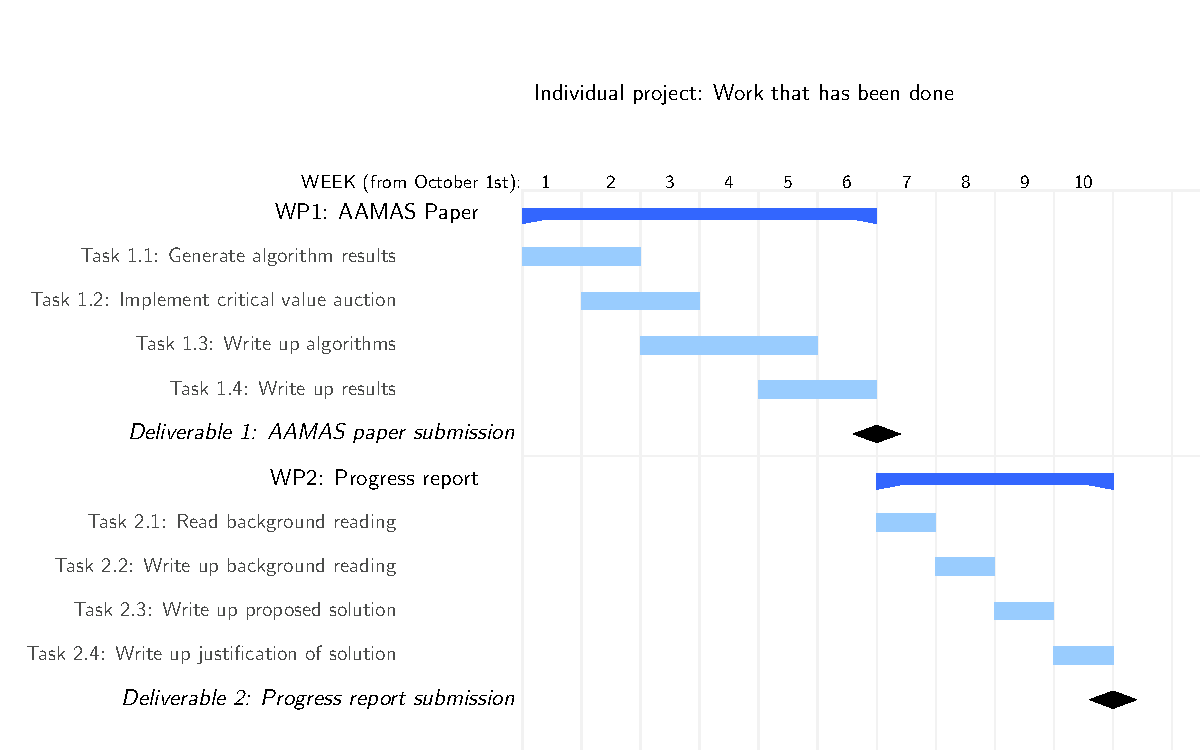
\includegraphics[width=\linewidth]{past_work_grantt/past_grantt.pdf}
    \caption{Work that has been done to date}
    \label{fig:past_grantt}
\end{figure}

\section{Plan of the remaining work}
Due to this term having been completing the paper (Section~\ref{sec:aamas_paper}), I have not done any programming
towards the project. Therefore the begin of the next term will be spend building the framework for which different pricing and
resource allocation heuristics can be applied and compared. Once this has been completed, analysis and comparison of
the heuristic will be done with different server and task models. Resulting in a final paper.
\begin{figure}[t]
    \centering
    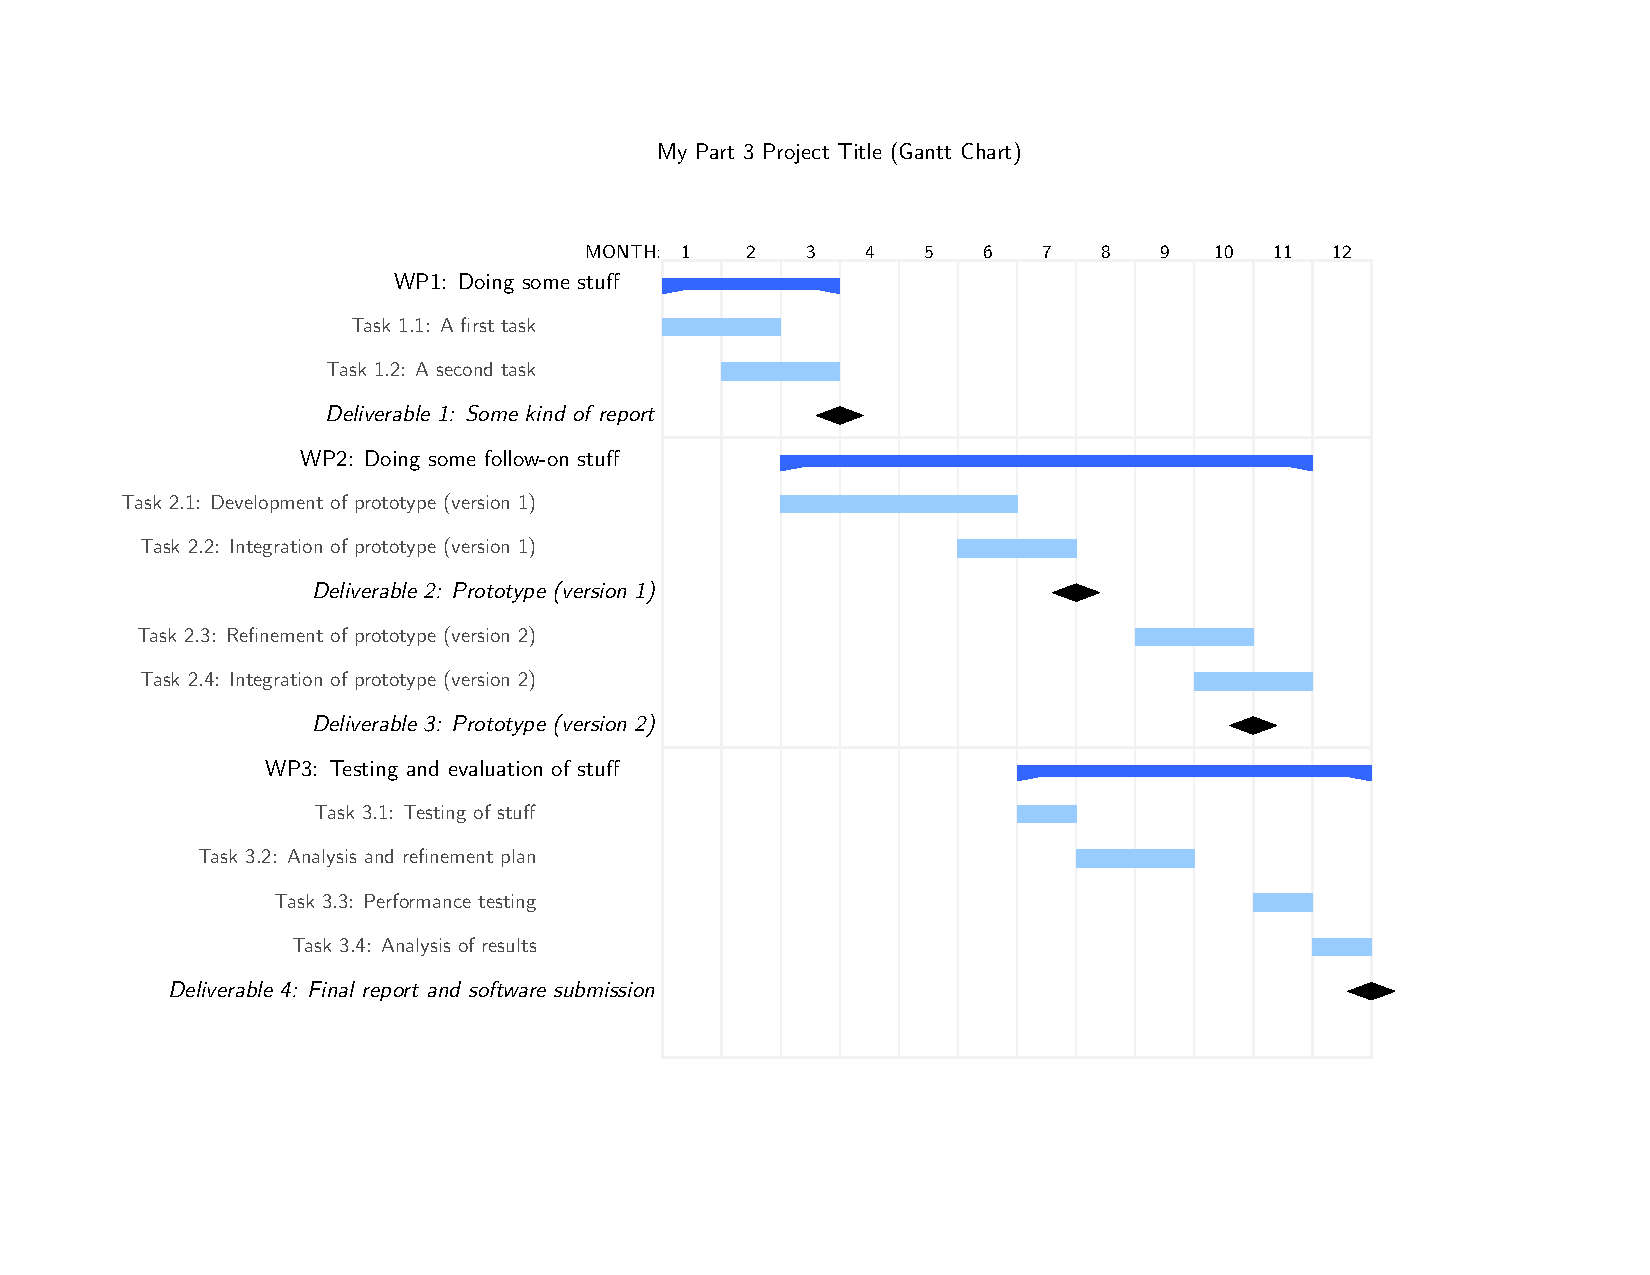
\includegraphics[width=\linewidth]{future_work_grantt/future_grantt}
    \caption{Work that will be done in the future}
    \label{fig:future_grantt}
\end{figure}